
软件项目都会直接或间接地使用多个代码存储库。处理本地项目代码最简单,但软件项目很少是独立的。若没有适当的依赖管理策略,事情可能会变得复杂。本章的第一个建议是若可以的话使用包管理器,包管理器大大减少了花费在依赖项管理上的工作。若不能使用包管理器,可能需要使用自己的迷你项目专用包管理器,这称为超级构建。

超级构建通常用于实现项目自给自足的依赖关系,所以项目能够在不需要用户干预的情况下满足依赖关系,拥有这样的能力对所有使用来说都非常方便。

\subsubsubsection{10.3.1\hspace{0.2cm}推荐的方法 – FetchContent}

我们将使用第10章01例进行演示,先从CMakeLists.txt文件开始。为了简单起见,省略了前七行:

\begin{lstlisting}[style=styleCMake]
if(CH10_EX01_USE_SUPERBUILD)
	include(superbuild.cmake)
else()
	find_package(GTest 1.10.0 REQUIRED)
	find_package(benchmark 1.6.1 REQUIRED)
endif()

add_executable(ch10_ex01_tests)
target_sources(ch10_ex01_tests PRIVATE src/tests.cpp)
target_link_libraries(ch10_ex01_tests PRIVATE GTest::Main)

add_executable(ch10_ex01_benchmarks)
target_sources(ch10_ex01_benchmarks PRIVATE src/benchmarks.cpp)
target_link_libraries(ch10_ex01_benchmarks PRIVATE benchmark::benchmark)
\end{lstlisting}

这是一个简单的CMakeLists.txt文件,定义了两个目标ch10\_ex01\_tests和ch10\_ex01\_benchmark。这些目标分别依赖于Google Test和Google Benchmark库。这些库可以通过超级构建或\texttt{find\_package(…)}调用找到和定义,这取决于CH10\_EX01\_USE\_SUPERBUILD变量。我们一直使用\texttt{find\_package(…)}确定路径,来看一下超级构建文件superbuild.cmake:

\begin{lstlisting}[style=styleCMake]
include(FetchContent)
FetchContent_Declare(benchmark
	GIT_REPOSITORY https://github.com/google/benchmark.git
	GIT_TAG v1.6.1
)
FetchContent_Declare(GTest
	GIT_REPOSITORY https://github.com/google/googletest.git
	GIT_TAG release-1.10.0
)

FetchContent_MakeAvailable(GTest benchmark)
add_library(GTest::Main ALIAS gtest_main)
\end{lstlisting}

第一行中,包含了\texttt{FetchContent}模块,使用它来获取依赖。接下来的六行中,\texttt{FetchContent\_Declare}用于声明两个外部目标,benchmark和GTest,并通过Git获取。因此,调用\texttt{FetchContent\_MakeAvailable(…)}使目标可用。最后,\texttt{add\_library(…)}用于为gtest\_main目标定义一个名为GTest::Main的别名目标。这样做是为了保持\texttt{find\_package(…)}和超级构建目标名称间的兼容性。因为\texttt{find\_package(…)}和超级构建目标名称已经兼容,所以没有为benchmark定义别名目标。

通过调用以下命令来配置和构建这个示例:

\begin{tcblisting}{commandshell={}}
cd chapter10/ex01_external_deps
cmake -S ./ -B build -DCH10_EX01_USE_SUPERBUILD:BOOL=ON
cmake --build build/ --parallel $(nproc)
\end{tcblisting}

在前两行中,进入example\_10/文件夹并配置项目。注意,这里CH10\_EX01\_USE\_SUPERBUILD为ON,以便启用超级构建代码。最后一行中,用N个并行作业构建项目,其中N是nproc的结果。

由于有了\texttt{find\_package(…)}的路径,若环境中的google test ≥ 1.10.0和google benchmark ≥ 1.6.1,那么构建也可以在不启用超级构建的情况下正常工作。这允许包维护人员在不打补丁的情况下更改依赖项版本。像这样的小型定制点对于可移植性和可重复性非常重要。

接下来,再来看一个使用ExternalProject模块的超级构建示例。

\subsubsubsection{10.3.2\hspace{0.2cm}传统的方式 – ExternalProject\_Add}

在\texttt{FetchContent}出现之前,大多数人会使用\texttt{ExternalProject\_Add}来实现超级构建方法。该功能由\texttt{ExternalProject}模块提供。本节中,将看到一个使用\texttt{ExternalProject\_Add}的超级构建示例,以了解它与\texttt{FetchContent}模块的区别。

来一起看看第10章中的CMakeLists.txt文件,示例02(省略了注释和项目指令):

\begin{lstlisting}[style=styleCMake]
# ...
include(superbuild.cmake)
add_executable(ch10_ex02_tests)
target_sources(ch10_ex02_tests PRIVATE src/tests.cpp)
target_link_libraries(ch10_ex02_tests PRIVATE catch2)
\end{lstlisting}

同样,该项目是一个包含单C++源文件的单元测试项目,但这次使用的是Catch2。CMakeLists.txt文件包括superbuild.cmake文件,定义一个可执行目标,并将Catch2库链接到目标。这个示例没有使用\texttt{FindPackage(…)}来查找Catch2库。与\texttt{FetchContent}不同,\texttt{ExternalProject}在构建时获取并构建外部依赖项。由于Catch2库的内容在配置时不可用,因此我们无法在这里使用\texttt{FindPackage(…)}。\texttt{FindPackage(…)}在配置时运行,并要求提供包文件。来看下superbuild.cmake:

\begin{lstlisting}[style=styleCMake]
include(ExternalProject)
ExternalProject_Add(catch2_download
	GIT_REPOSITORY https://github.com/catchorg/Catch2.git
	GIT_TAG v2.13.9
	INSTALL_COMMAND ""
	# For disabling the warning that treated as an error
	CMAKE_ARGS -DCMAKE_CXX_FLAGS="-Wno-error=pragmas"
)
SET(CATCH2_INCLUDE_DIR ${CMAKE_CURRENT_BINARY_DIR}
	/catch2_download-prefix/src/catch2_download/single_include)
file(MAKE_DIRECTORY ${CATCH2_INCLUDE_DIR})
add_library(catch2 IMPORTED INTERFACE GLOBAL)
add_dependencies(catch2 catch2_download)
set_target_properties(catch2 PROPERTIES
	"INTERFACE_INCLUDE_DIRECTORIES" "${CATCH2_INCLUDE_DIR}")
\end{lstlisting}

superbuild.cmake模块包括\texttt{ExternalProject}模块,使用\texttt{ExternalProject\_Add},用GIT\_REPOSITORY、GIT\_TAG、INSTALL\_COMMAND和CMAKE\_ARGS参数声明一个名为catch2\_download的目标。\texttt{ExternalProject\_Add}可以从不同的源获取依赖项,示例试图通过使用Git获取依赖项。GIT\_REPOSITORY和GIT\_TAG参数分别用于指定目标git库URL和在git克隆后要检出的标记。因为Catch2是一个CMake项目,需要提供给\texttt{ExternalProject\_Add}的参数量最小。\texttt{ExternalProject\_Add}默认知道如何配置、构建和安装CMake项目,因此不需要CONFIGURE\_COMMAND或BUILD\_COMMAND参数。空的INSTALL\_COMMAND参数用于在构建之后禁用并安装依赖项。最后一个参数,CMAKE\_ARGS,用于将CMAKE参数传递给外部项目的配置步骤。我们使用它来静默关于Catch2编译中的语法警告(作为错误处理)。

\texttt{ExternalProject\_Add}将所需的库获取到前缀路径中并构建,要使用获取的内容,必须首先将其导入到项目中。因为不能使用\texttt{FindPackage(…)}进行导入,所以需要手动做一些工作,其中之一是定义Catch2目标的include目录。因为Catch2是一个纯头文件库,所以用头文件定义一个接口目标就够了。这里声明了CATCH2\_INCLUDE\_DIR变量来设置将包含CATCH2头文件的目录,使用这个变量来设置本例中创建的导入目标的INTERFACE\_INCLUDE\_DIRECTORIES属性。接下来,使用\texttt{file (MAKE\_DIRECTORY \$\{CATCH2\_INCLUDE\_DIR\})}指令来创建include目录。由于ExternalProject\_Add的工作方式,在执行构建步骤之前不会出现Catch2内容。设置一个目标的INTERFACE\_INCLUDE\_DIRECTORIES需要给定的目录存在,所以使用了一个小hack作为解决方案。最后三行中,为Catch2声明一个导入的INTERFACE库,使这个库依赖于catch2\_download目标,并设置导入库的INTERFACE\_INCLUDE\_DIRECTORIES。

试着配置和构建来检查以上设置是否有效:

\begin{tcblisting}{commandshell={}}
cd chapter10/ex02_external_deps_with_extproject
cmake -S ./ -B build
cmake --build build/ --parallel $(nproc)
\end{tcblisting}

若一切正常,会看到类似这样的输出:

\begin{tcblisting}{commandshell={}}
[ 10%] Creating directories for 'catch2_download'
[ 20%] Performing download step (git clone) for
  'catch2_download'
Cloning into 'catch2_download'...
HEAD is now at 62fd6605 v2.13.9
[ 30%] Performing update step for 'catch2_download'
[ 40%] No patch step for 'catch2_download'
[ 50%] Performing configure step for 'catch2_download'
/* ... */
[ 60%] Performing build step for 'catch2_download'
/* ... */
[ 70%] No install step for 'catch2_download'
[ 80%] Completed 'catch2_download'
[ 80%] Built target catch2_download
/* ... */
[100%] Built target ch10_ex02_tests
\end{tcblisting}

好了,似乎已经成功构建了测试可执行文件。通过运行./build/ch10\_ex02\_tests可执行文件来检查它是否有效:

\begin{tcblisting}{commandshell={}}
===========================================================
All tests passed (4 assertions in 1 test case)
\end{tcblisting}

接下来,了解如何在超级构建中使用QT框架,并创建简单的QT应用程序。

\subsubsubsection{10.3.3\hspace{0.2cm}福利 - 超级构建中使用Qt 6框架}

我们处理的都是体积相当小的库。来试试一些更复杂的东西,比如在超级构建中使用一个大框架,比如Qt框架。对于这一部分,我们将使用第10章,示例03的例子。

\begin{tcolorbox}[colback=yellow!5!white,colframe=yellow!75!black,title=重要的Note]
若打算在提供的Docker容器之外尝试这个示例,可能必须安装Qt运行时所需的一些附加依赖项。类Debian系统所需的包如下:libgl1-mesa-dev libglu1-mesa-dev '\^{}libxcb.*-dev' libx11-xcb-dev libglu1-mesa-dev libxrender-dev libxi-dev libxkbcommon-dev libxkbcommon-x11-dev。
\end{tcolorbox}

该示例包含一个源文件main.cpp,输出一个简单的Qt窗口应用程序和一条消息:

\begin{lstlisting}[style=styleCXX]
#include <qapplication.h>
#include <qpushbutton.h>
int main( int argc, char **argv )
{
	QApplication a( argc, argv );
	QPushButton hello( "Hello from CMake Best Practices!",
	0 );
	hello.resize( 250, 30 );
	hello.show();
	return a.exec();
}
\end{lstlisting}

我们的目标是能够编译这个Qt应用程序,而不需要用户自己安装Qt框架。超级构建应该会自动安装Qt 6,应用程序应该能够使用该框架。先看一下这个例子的CMakeLists.txt:

\begin{lstlisting}[style=styleCMake]
if(CH10_EX03_USE_SUPERBUILD)
	include(superbuild.cmake)
else()
	set(CMAKE_AUTOMOC ON)
	set(CMAKE_AUTORCC ON)
	set(CMAKE_AUTOUIC ON)

	find_package(Qt6 COMPONENTS Core Widgets REQUIRED)
endif()

add_executable(ch10_ex03_simple_qt_app main.cpp)
target_compile_features(ch10_ex03_simple_qt_app PRIVATE cxx_std_11)
target_link_libraries(ch10_ex03_simple_qt_app Qt6::Core Qt6::Widgets)
\end{lstlisting}

与第一个示例类似,CMakeLists.txt文件包括superbuild.cmake文件,取决于选项标志。若用户选择为该示例使用超级构建,那么将包括超级构建模块。否则,依赖将尝试使用\texttt{find\_package(…)}在系统中定位。最后三行中,定义了一个可执行目标,设置了目标的C++标准,并将定义的目标链接到Qt6::Core和Qt6::Widgets目标。这些目标要么由超级构建定义,要么由\texttt{find\_package(…)}定义,这取决于用户是否选择使用超级构建。继续来看superbuild.cmake:

\begin{lstlisting}[style=styleCMake]
include(FetchContent)
message(STATUS "Chapter 10, example 03 superbuild enabled.
	Will try to satisfy dependencies for the example.")
# Enable message output for FetchContent commands
set(FETCHCONTENT_QUIET FALSE)
set(QT_BUILD_SUBMODULES "qtbase" CACHE STRING "Submodules to build")
set(QT_WILL_BUILD_TOOLS on)
set(QT_FEATURE_sql off)
set(QT_FEATURE_network off)
set(QT_FEATURE_dbus off)
set(QT_FEATURE_opengl off)
set(QT_FEATURE_testlib off)
set(QT_BUILD_STANDALONE_TESTS off)
set(QT_BUILD_EXAMPLES off)
set(QT_BUILD_TESTS off)

FetchContent_Declare(qt6
	GIT_REPOSITORY https://github.com/qt/qt5.git
	GIT_TAG v6.3.0
	GIT_SHALLOW TRUE
	GIT_PROGRESS TRUE # Since the clone process is lengthy,
		show progress of download
	GIT_SUBMODULES qtbase # The only QT submodule we need
)
FetchContent_MakeAvailable(qt6)
\end{lstlisting}

superbuild.cmake文件使用\texttt{FetchContent}模块来获取Qt依赖。由于Qt的获取和准备过程可能很长,一些未使用的Qt框架特性会禁用。为了更好地跟踪进度,启用了\texttt{FetchContent}消息输出。让我们试着通过运行以下命令来配置和编译这个示例:

\begin{tcblisting}{commandshell={}}
cd chapter10/ex03_simple_qt_app/
cmake -S ./ -B build -DCH10_EX03_USE_SUPERBUILD:BOOL=ON
cmake --build build/ --parallel $(nproc)
\end{tcblisting}

若一切顺利,应该会看到类似的输出:

\begin{tcblisting}{commandshell={}}
/*...*/
[ 11%] Creating directories for 'qt6-populate'
[ 22%] Performing download step (git clone) for
  'qt6-populate'
Cloning into 'qt6-src'...
/*...*/
[100%] Completed 'qt6-populate'
[100%] Built target qt6-populate
/*...*/
-- Configuring done
-- Generating done
/*...*/
[ 0%] Generating ../../mkspecs/modules
\end{tcblisting}
\begin{tcblisting}{commandshell={}}
  /qt_lib_widgets_private.pri
[ 0%] Generating ../../mkspecs/modules
/qt_lib_gui_private.pri
[ 0%] Generating ../../mkspecs/modules/qt_lib_core_private.pri
/* ... */
[ 98%] Linking CXX executable ch10_ex03_simple_qt_app
[ 98%] Built target ch10_ex03_simple_qt_app
/*...*/
\end{tcblisting}

一切顺利!让我们用以下命令运行生成的可执行文件来检查它是否工作:

\begin{tcblisting}{commandshell={}}
./build/ch10_ex03_simple_qt_app
\end{tcblisting}

一切正常的话,应该会弹出一个小GUI窗口:

\begin{center}
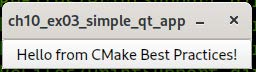
\includegraphics[width=0.4\textwidth]{content/2/chapter10/images/1.jpg}\\
图10.1 简单的Qt应用程序窗口
\end{center}

我们已经完成了学习如何在CMake项目中使用超级构建。接下来,来看看如何在超级构建中保持版本一致性。

















